\section{Literate Programming}
\label{sec:literate-programming}

Literate programming was first introduced in 1984 for the Pascal programming
language~\cite{knuth1984}. Even though the idea was conceived over 30 years
ago, implementations are not very common. In recent years the idea seems to
gain popularity again. Examples include the IPython project~\cite{ipython2007},
published in 2007, as well as Swift Playgrounds~\cite{swift-playgrounds},
introduced in 2014.

Just as with REPLs, the concept of literate programming is known by various
names in slightly different forms. This section starts with an explanation of
what literate programming is exactly.

According to Donald Knuth, better documentation of programs is essential to make
further progress in the state of the art of programming.
To achieve this he proposes to write programs not with the intention to
explain the computer what to do, but with the intention to explain to humans
what the programmer wants a computer to do~\cite{knuth1984},
by mixing documentation and code in a single source file.
This idea of literate programming was realized in its original form as the
`WEB' language developed during Knuth's research at Stanford University.

\subsubsection{The `WEB' language}

The `WEB' language was mainly a combination of two other languages, namely
\TeX{} for document formatting and PASCAL as the programming language. By
combining these languages, each with a different purpose, into one language, the
source code serves two purposes: to produce a document describing the program
and to produce a machine-executable program. Since both program and
documentation are generated from the same source file, they are always
consistent with each other.

\subsubsection{IPython / Jupyter notebooks}

A more recent example of literate programming comes in the form of IPython with
Jupyter notebooks~\cite{ipython2007}. IPython was partially inspired by other
scientific tools already offering notebook-like functionality, such as Matlab or
Mathematica. Besides the literal programming style introduced by `WEB', IPython
notebooks allow for REPL-style interactive editing; documentation and code can
be edited live and blocks of code can be reevaluated, printing their updated
results. IPython notebooks also allow for more complex graphical elements such
as 3D-plots. See \cref{fig:ipython} for an example of an IPython notebook.

\begin{figure}[htb]
  \centering
  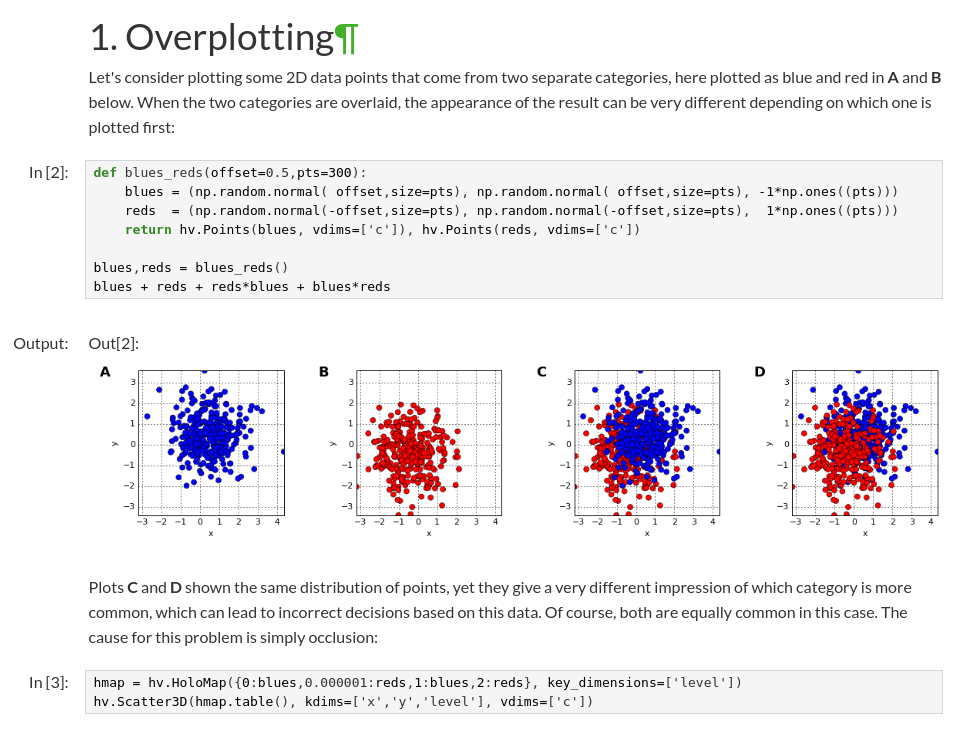
\includegraphics[width=\textwidth]{ipython}
  \caption{A plot from data in an IPython notebook.}
  \label{fig:ipython}
\end{figure}

%%% Local Variables:
%%% mode: latex
%%% TeX-master: "main"
%%% End:
